
%(BEGIN_QUESTION)
% Copyright 2006, Tony R. Kuphaldt, released under the Creative Commons Attribution License (v 1.0)
% This means you may do almost anything with this work of mine, so long as you give me proper credit

The principle of buoyancy may be used to create a level transmitter instrument, generating an output signal proportional to the change in weight of a ``displacer'' rod suspended in a liquid:

$$\includegraphics[width=15.5cm]{i00276x01.eps}$$

Often, the displacer is housed inside its own ``cage'' for easy removal from the process, as shown above, or it may be inserted directly into the process vessel like this:

$$\includegraphics[width=15.5cm]{i00276x02.eps}$$

If the vessel is open and the liquid inside is turbulent due to mixing or other agitation, a {\it stilling well} serves the same purpose as a cage:

$$\includegraphics[width=15.5cm]{i00276x03.eps}$$

To calibrate such an instrument, it must be isolated from the process liquid.  Sometimes this means simply closing block valves and draining the cage.  Other times it means removing the displacer mechanism from the vessel entirely.  But once the displacer is hanging dry, there is the problem of simulating a 100\% condition for calibration purposes.

Describe a way to make the displacer ``think'' it is fully submerged in process liquid when it in fact is hanging freely in the air.  Explain how you would be able to {\it precisely} and {\it accurately} simulate this condition, as well as any given condition of partial displacer submersion for that matter.

\underbar{file i00276}
%(END_QUESTION)





%(BEGIN_ANSWER)

One way to simulate a full condition is to use a {\it hand scale}:

$$\includegraphics[width=15.5cm]{i00276x04.eps}$$

%(END_ANSWER)





%(BEGIN_NOTES)


%INDEX% Measurement, level: displacer (buoyancy)

%(END_NOTES)


